\newpage
\problem{layer\_norm\_ablation}{Remove RMSNorm and train}{1}

\textbf{Common protocol for the four ablations.}
I used TinyStories and the low-resource configuration: vocabulary 10,000,
context length 256, four layers, width 512, 16 heads, and batch size 16.
Each full run started from scratch with seed 42 and trained for 10,000 updates
(40.96M tokens) on MPS. AdamW used $\beta=(0.9,0.999)$, weight decay 0.1,
and gradient clipping at 1.0. After 100 warmup updates, the learning rate
followed cosine decay from $10^{-3}$ to $10^{-4}$, except for the reduced-LR
no-RMSNorm run described below. The baseline used pre-RMSNorm, RoPE, and
SwiGLU with hidden width 1,344.

For these comparisons I trained a fresh baseline and evaluated every 100
updates on the same 20 batches of 16 validation windows (81,920 tokens),
using a private generator reset to seed 42 at each evaluation. Validation
therefore did not consume the training sampler's random state. This protocol
differs from the earlier LR sweep's random validation sampling, so I use the
new baseline throughout this section rather than directly comparing its loss
with the older baseline. Figures are exported from W\&B panels with smoothing disabled.
Training loss is the current minibatch loss logged every ten updates;
validation loss uses the fixed windows described above.
All five full runs completed with finite logged losses and finite final model
weights; their final checkpoints also gave their best sampled validation losses.

\begin{table}[H]
    \centering
    \small
    \begin{tabular}{@{}lrrrr@{}}
        \toprule
        Model & Peak LR & Parameters & Final val loss & $\Delta$ vs. baseline \\
        \midrule
        Baseline & $10^{-3}$ & 22,696,448 & \textbf{1.5879} & --- \\
        No RMSNorm & $5\times10^{-4}$ & 22,691,840 & 1.6598 & $+0.0719$ \\
        Post-norm & $10^{-3}$ & 22,696,448 & 1.6042 & $+0.0163$ \\
        NoPE & $10^{-3}$ & 22,696,448 & 1.7010 & $+0.1131$ \\
        SiLU & $10^{-3}$ & 22,827,520 & 1.6106 & $+0.0227$ \\
        \bottomrule
    \end{tabular}
    \caption{Matched-budget ablation results at step 10,000. Lower validation
    cross-entropy is better. All runs use one seed; no-RMSNorm also changes LR.}
    \label{tab:ablation_results}
\end{table}

\textbf{Removing normalization and selecting a learning rate.}
I removed every RMSNorm, including the final normalization before the output
projection. At the previously selected peak LR $10^{-3}$, an early probe
with the 10,000-step schedule became unstable: validation loss reached 7.4620
at update 300 and 2125.2192 at update 400, before recovering to 2.4755 at
update 1,000. The values remained finite; this was a transient loss explosion,
not persistent unbounded divergence. This probe was stopped early and is not
a full-budget result.

I then screened peaks $3\times10^{-4}$ and $5\times10^{-4}$ with the same
long schedule. Neither showed comparable spikes in the logged window;
$5\times10^{-4}$ had lower loss at all ten corresponding evaluations,
ending at 2.4873 versus 2.5967 at update 1,000. I selected
$5\times10^{-4}$ with floor $5\times10^{-5}$ for a fresh full run.
This is the selected stable candidate among the short screens, rather than
a proven full-budget optimum.

\begin{figure}[H]
    \centering
    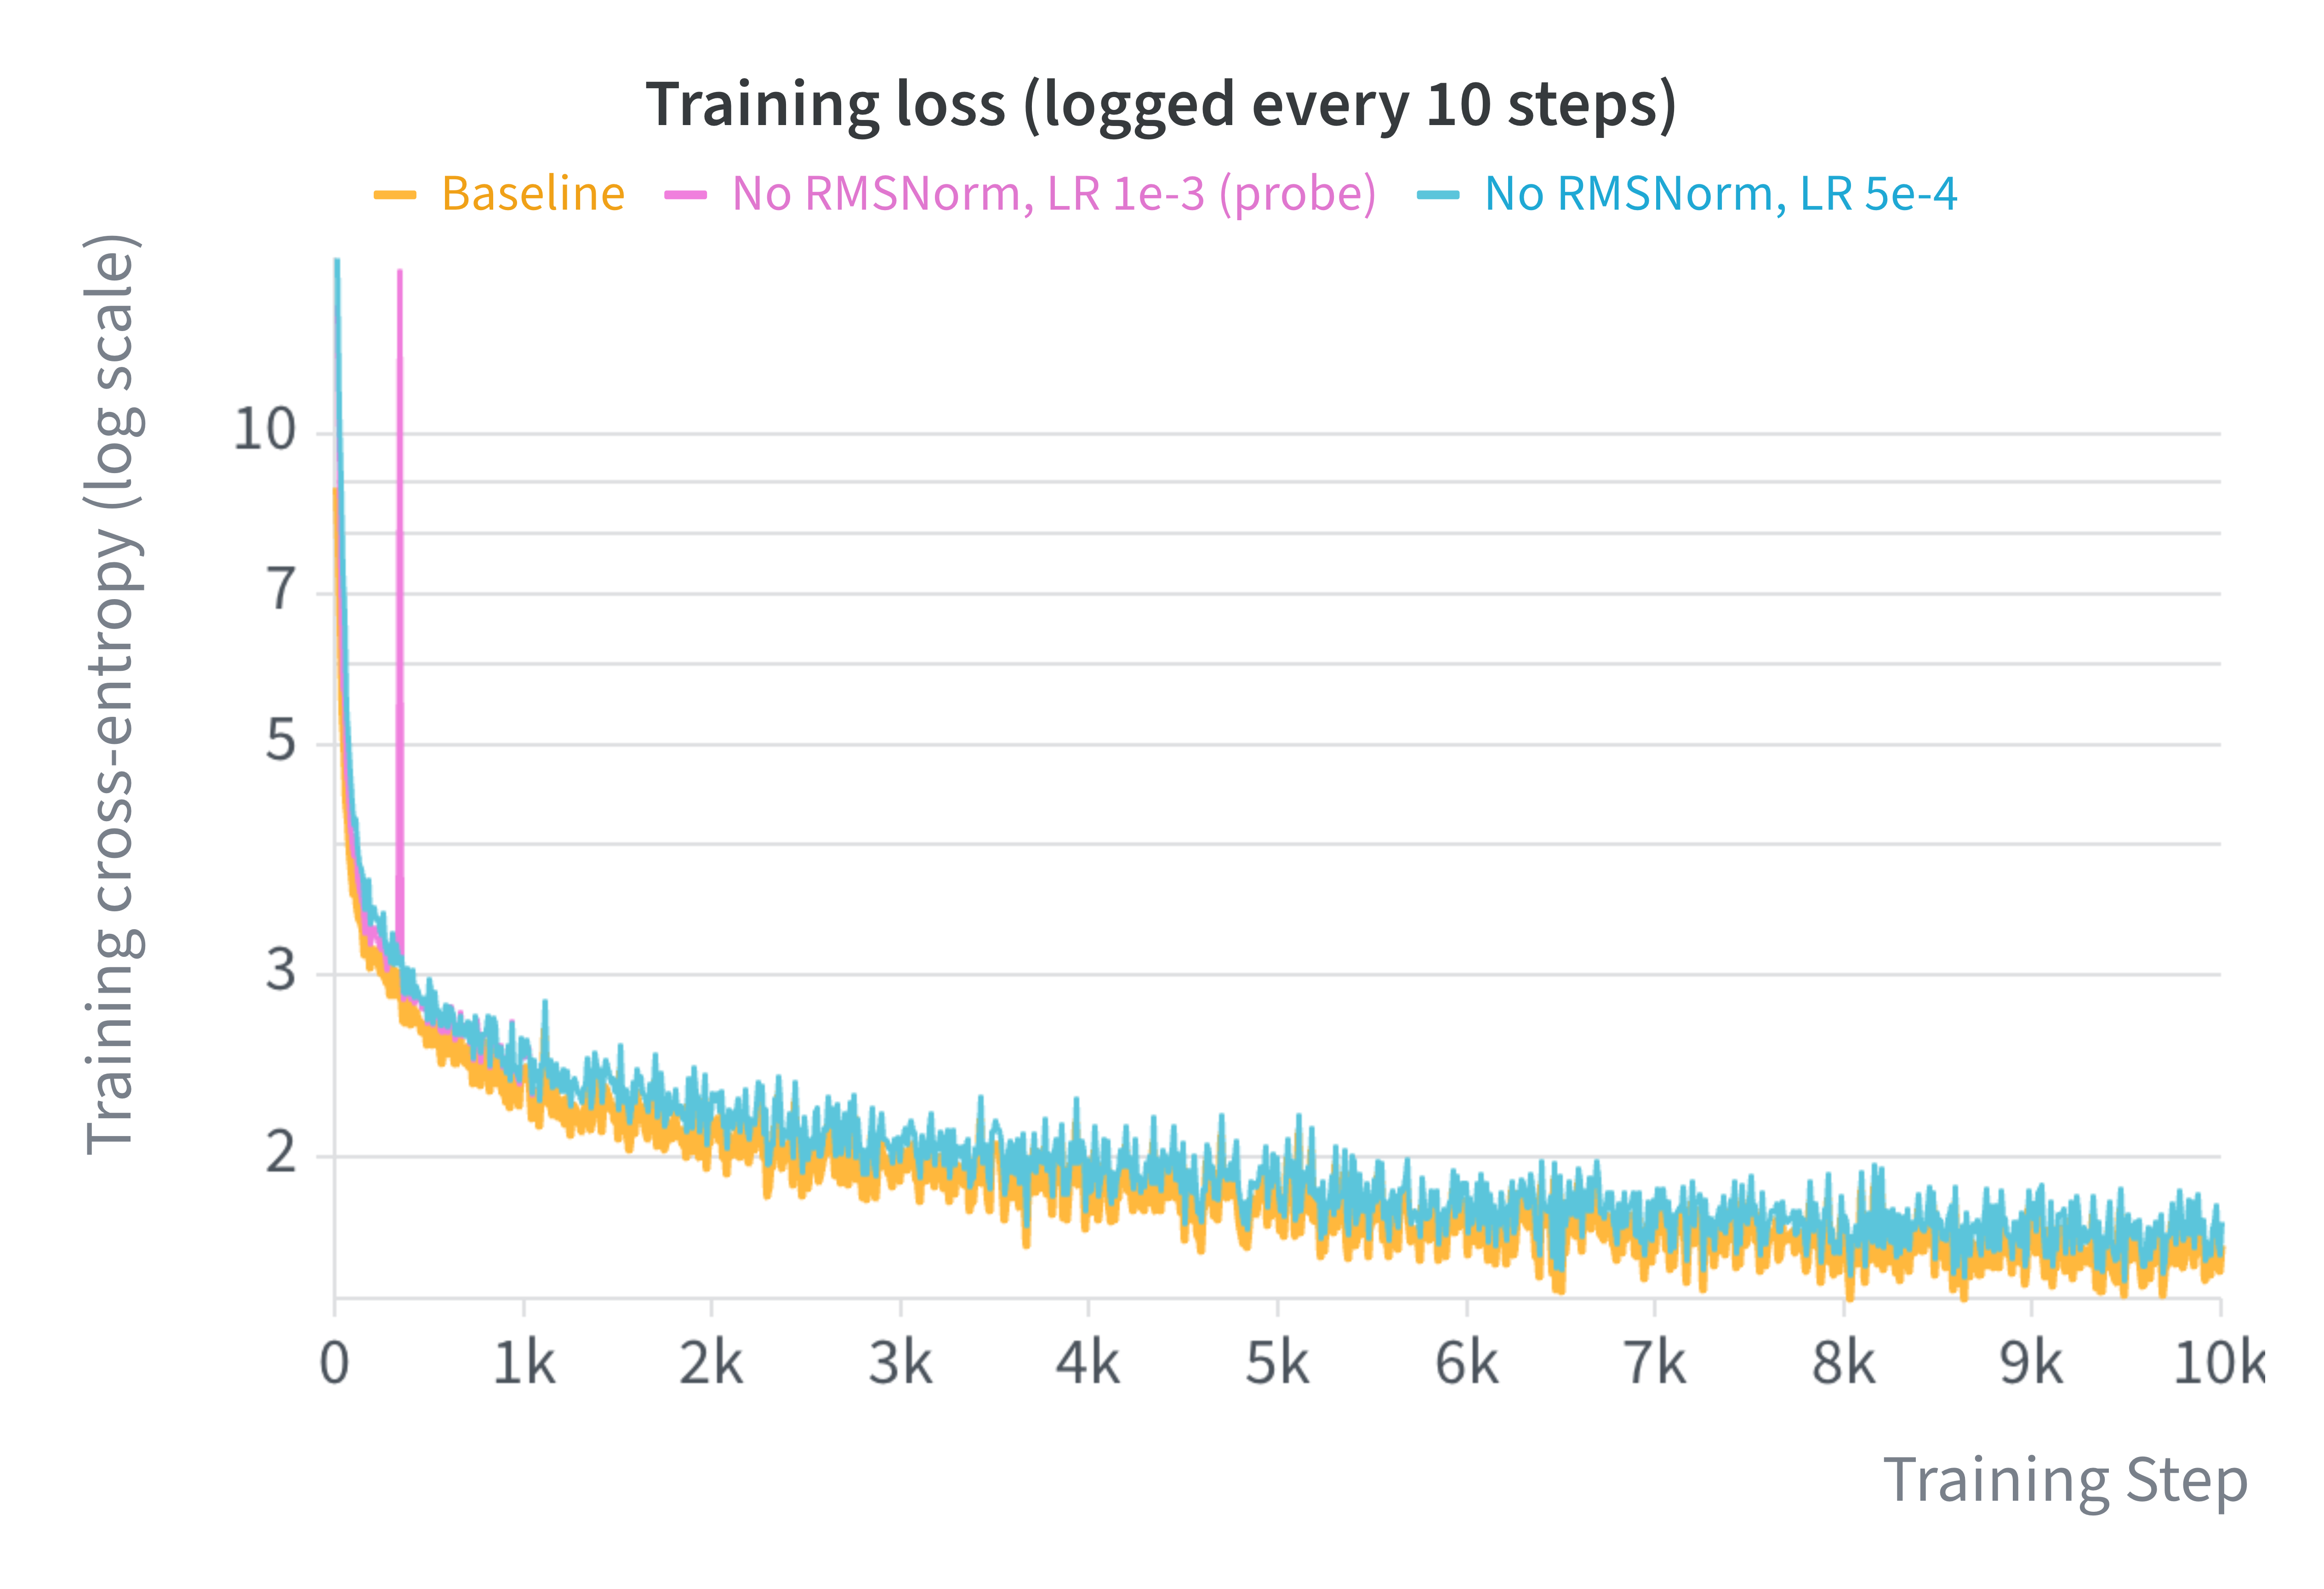
\includegraphics[width=0.49\textwidth]{figures/rmsnorm_train.png}\hfill
    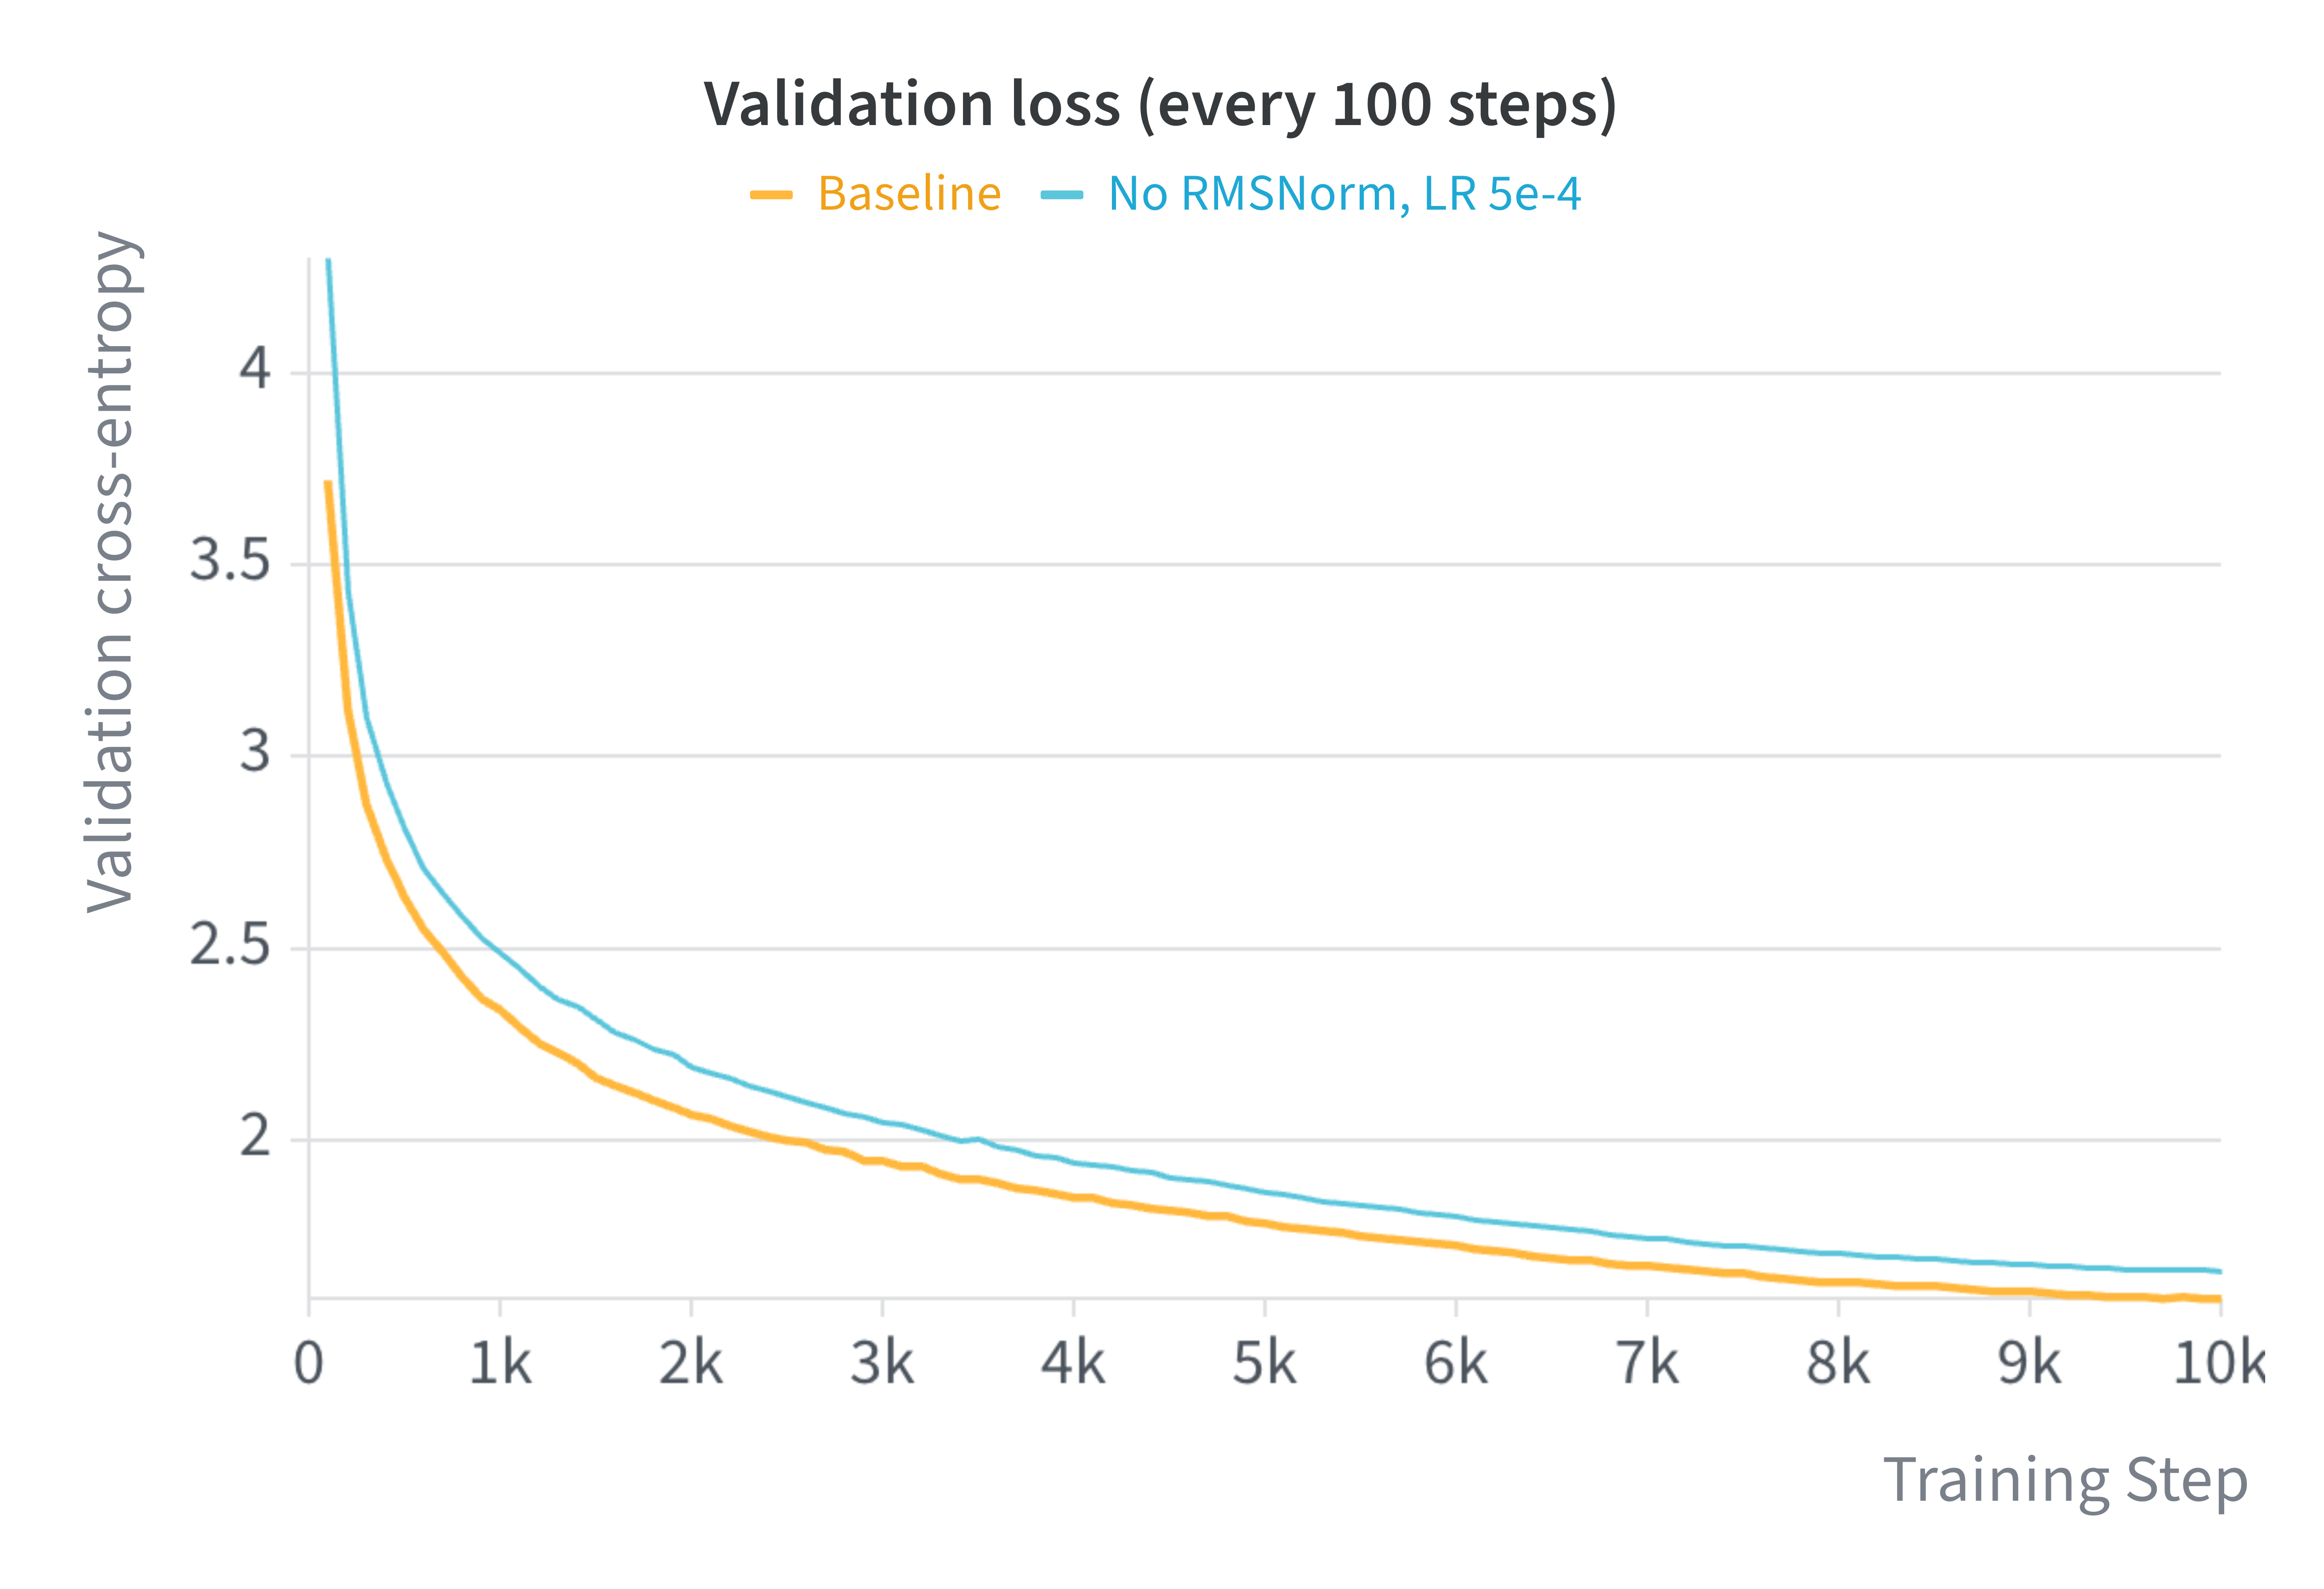
\includegraphics[width=0.49\textwidth]{figures/rmsnorm_val.png}
    \caption{RMSNorm ablation: W\&B training loss (left, logarithmic loss axis)
    and validation loss (right, linear loss axis). The training panel includes
    the early $10^{-3}$ no-RMSNorm probe, which ends near update 1,000;
    the validation panel compares only the complete baseline and reduced-LR
    no-RMSNorm runs. Legends give peak LR; floors are one tenth of peak.}
    \label{fig:layer_norm_ablation}
\end{figure}

The reduced-LR full run remained stable at the logged evaluations and reached
1.6598, compared with 1.5879 for the baseline. Its validation loss was higher
at all 100 matched evaluation points. Thus, normalization allowed stable
training at the larger tested LR, while reducing LR made training without
normalization practical in this setting. The final gap of 0.0719 reflects
both the architecture and the different LR schedule; it does not isolate the
causal effect of RMSNorm alone.

\newpage
\problem{pre\_norm\_ablation}{Implement post-norm and train}{1}

I moved each block's two RMSNorms after its attention and feed-forward
residual additions, retaining the final model RMSNorm. Model size, learning
rate, and the remaining common settings were unchanged.

\begin{figure}[H]
    \centering
    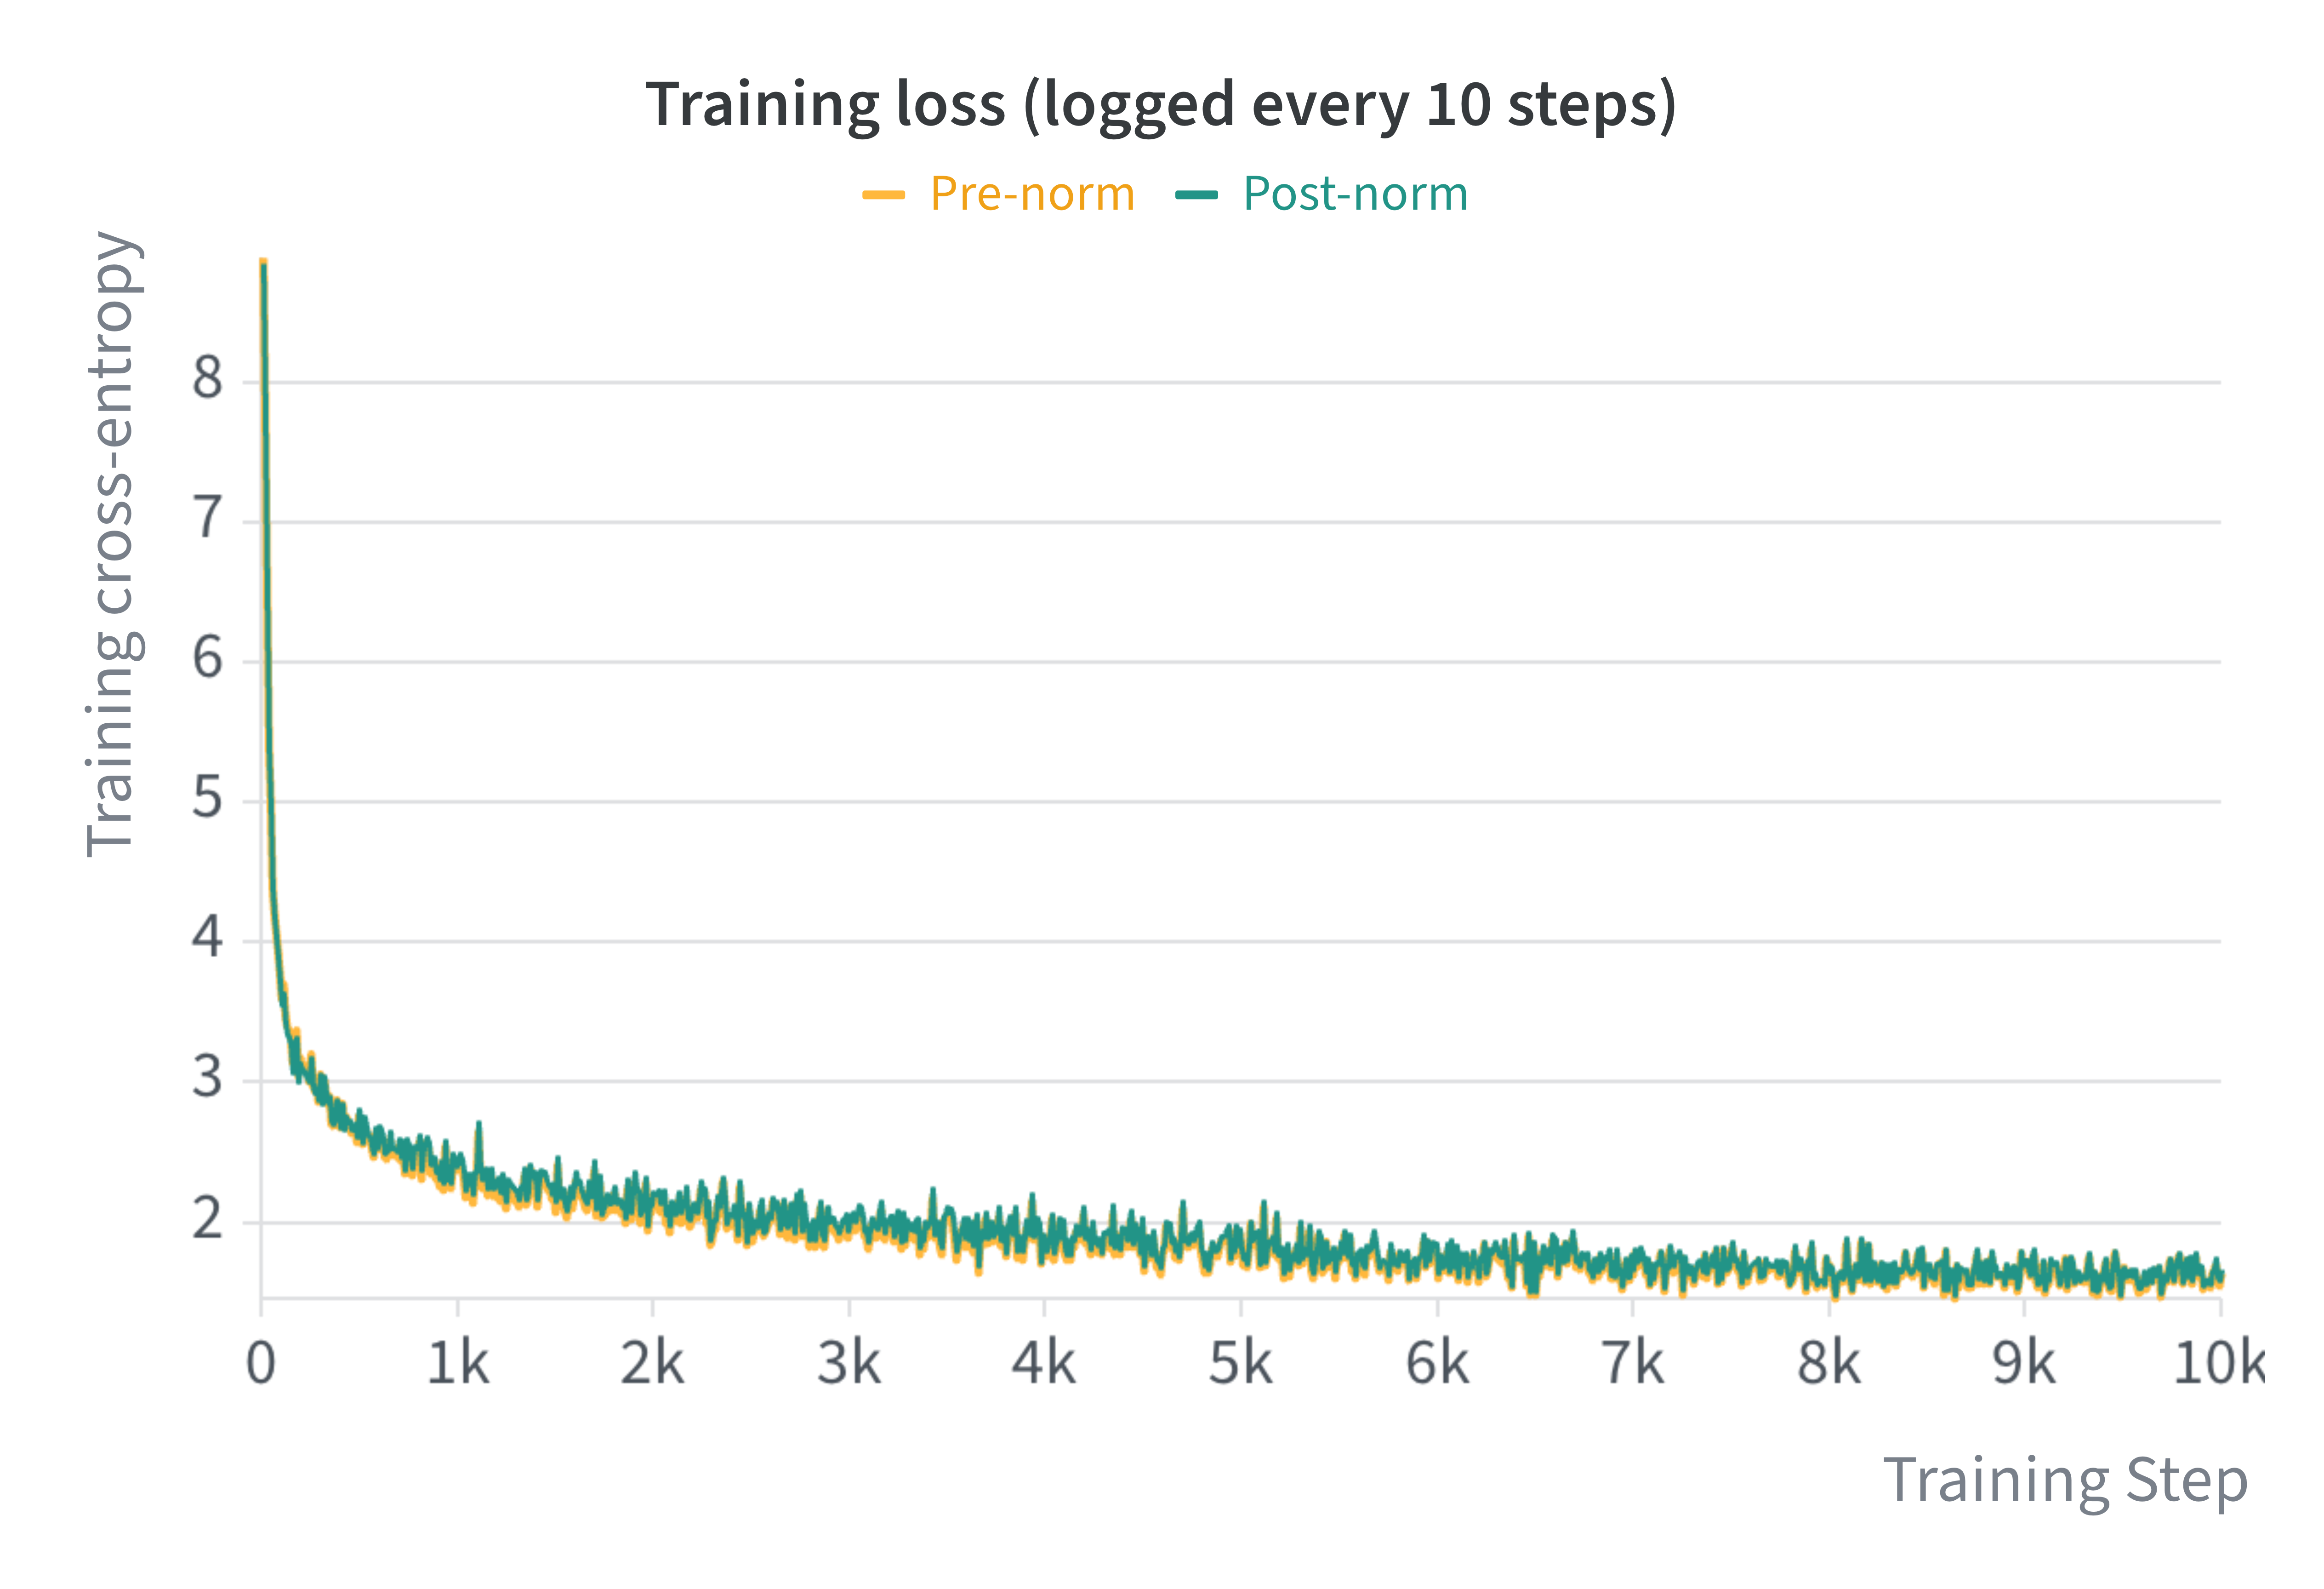
\includegraphics[width=0.49\textwidth]{figures/pre_post_norm_train.png}\hfill
    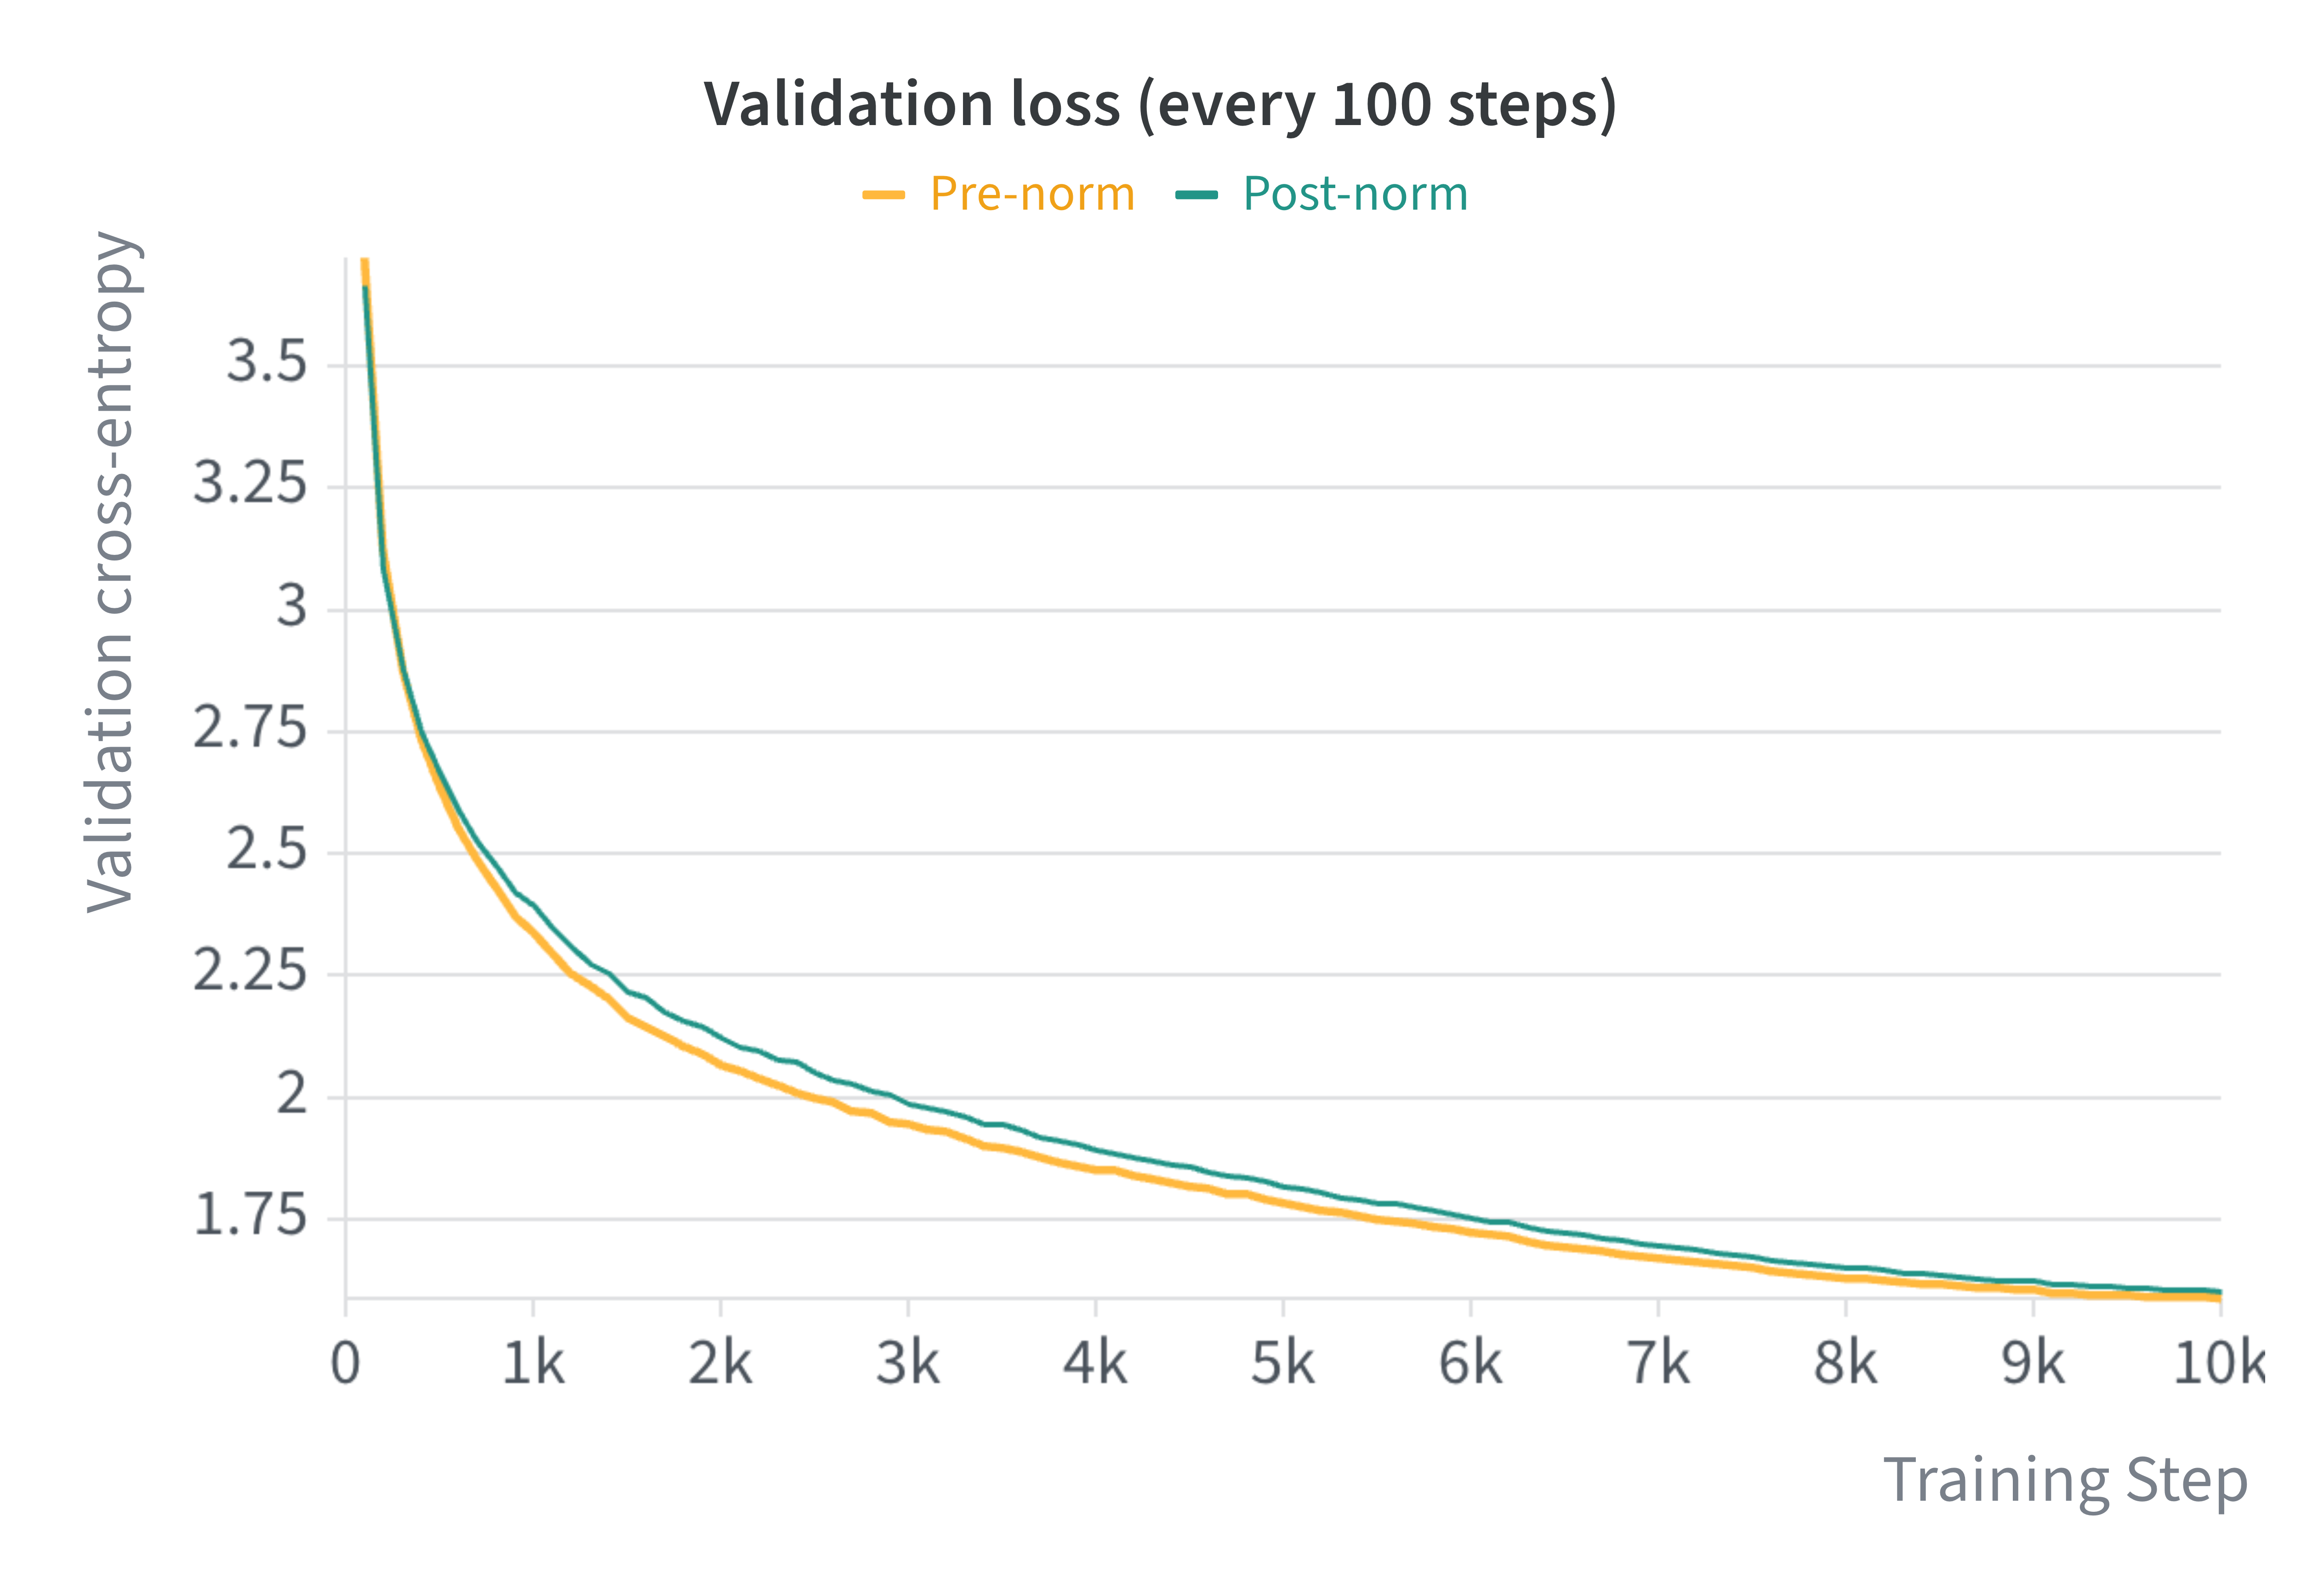
\includegraphics[width=0.49\textwidth]{figures/pre_post_norm_val.png}
    \caption{Pre-norm versus post-norm W\&B training loss (left) and validation
    loss (right), both at peak LR $10^{-3}$. Both panels cover the full run.}
    \label{fig:pre_norm_ablation}
\end{figure}

Both variants trained without comparable loss explosions. Post-norm was
slightly better at the first two evaluations, but had higher validation loss
at the remaining 98 evaluations. It ended at 1.6042 versus 1.5879 for
pre-norm, a gap of 0.0163. Pre-norm therefore performed slightly better
under this shared schedule; post-norm was still trainable in this four-layer
model. This single-seed comparison does not establish that post-norm is
inherently unstable or that the small final gap is statistically significant.

\problem{no\_pos\_emb}{Implement NoPE}{1}

I removed RoPE from every attention layer while retaining the causal mask.
This changes no trainable parameter counts; all other common settings,
including the LR schedule, were fixed.

\begin{figure}[H]
    \centering
    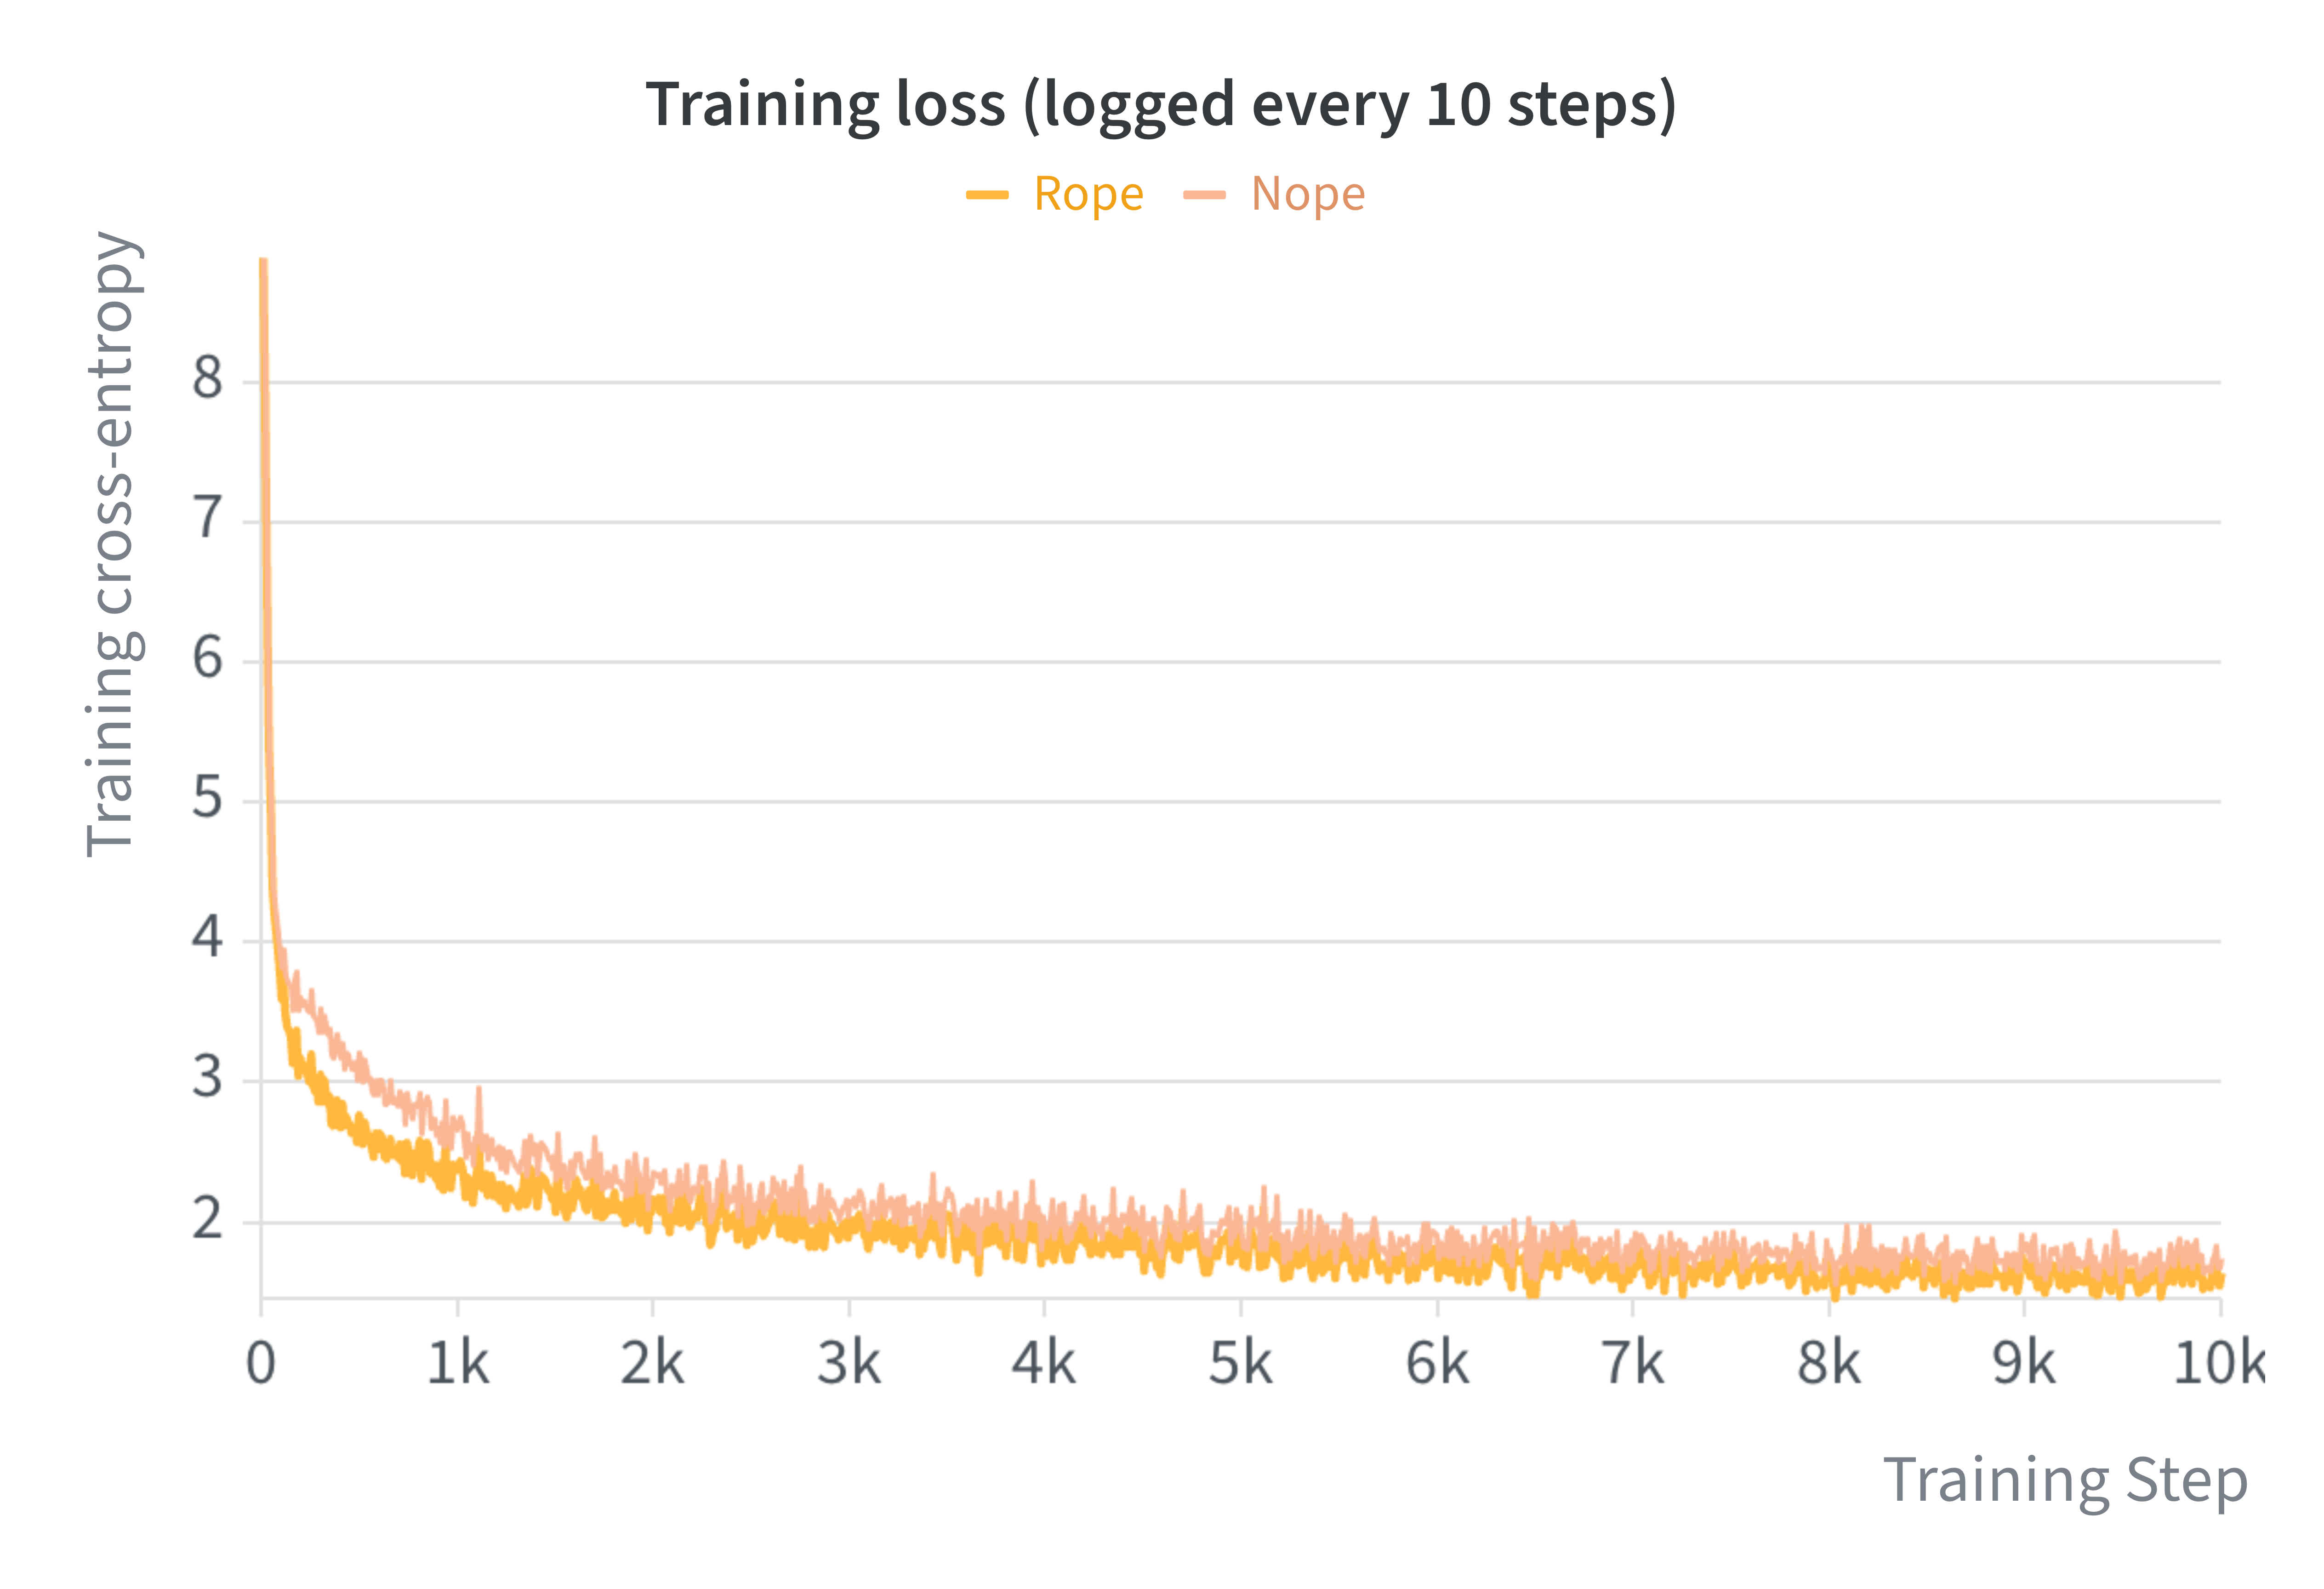
\includegraphics[width=0.49\textwidth]{figures/rope_nope_train.png}\hfill
    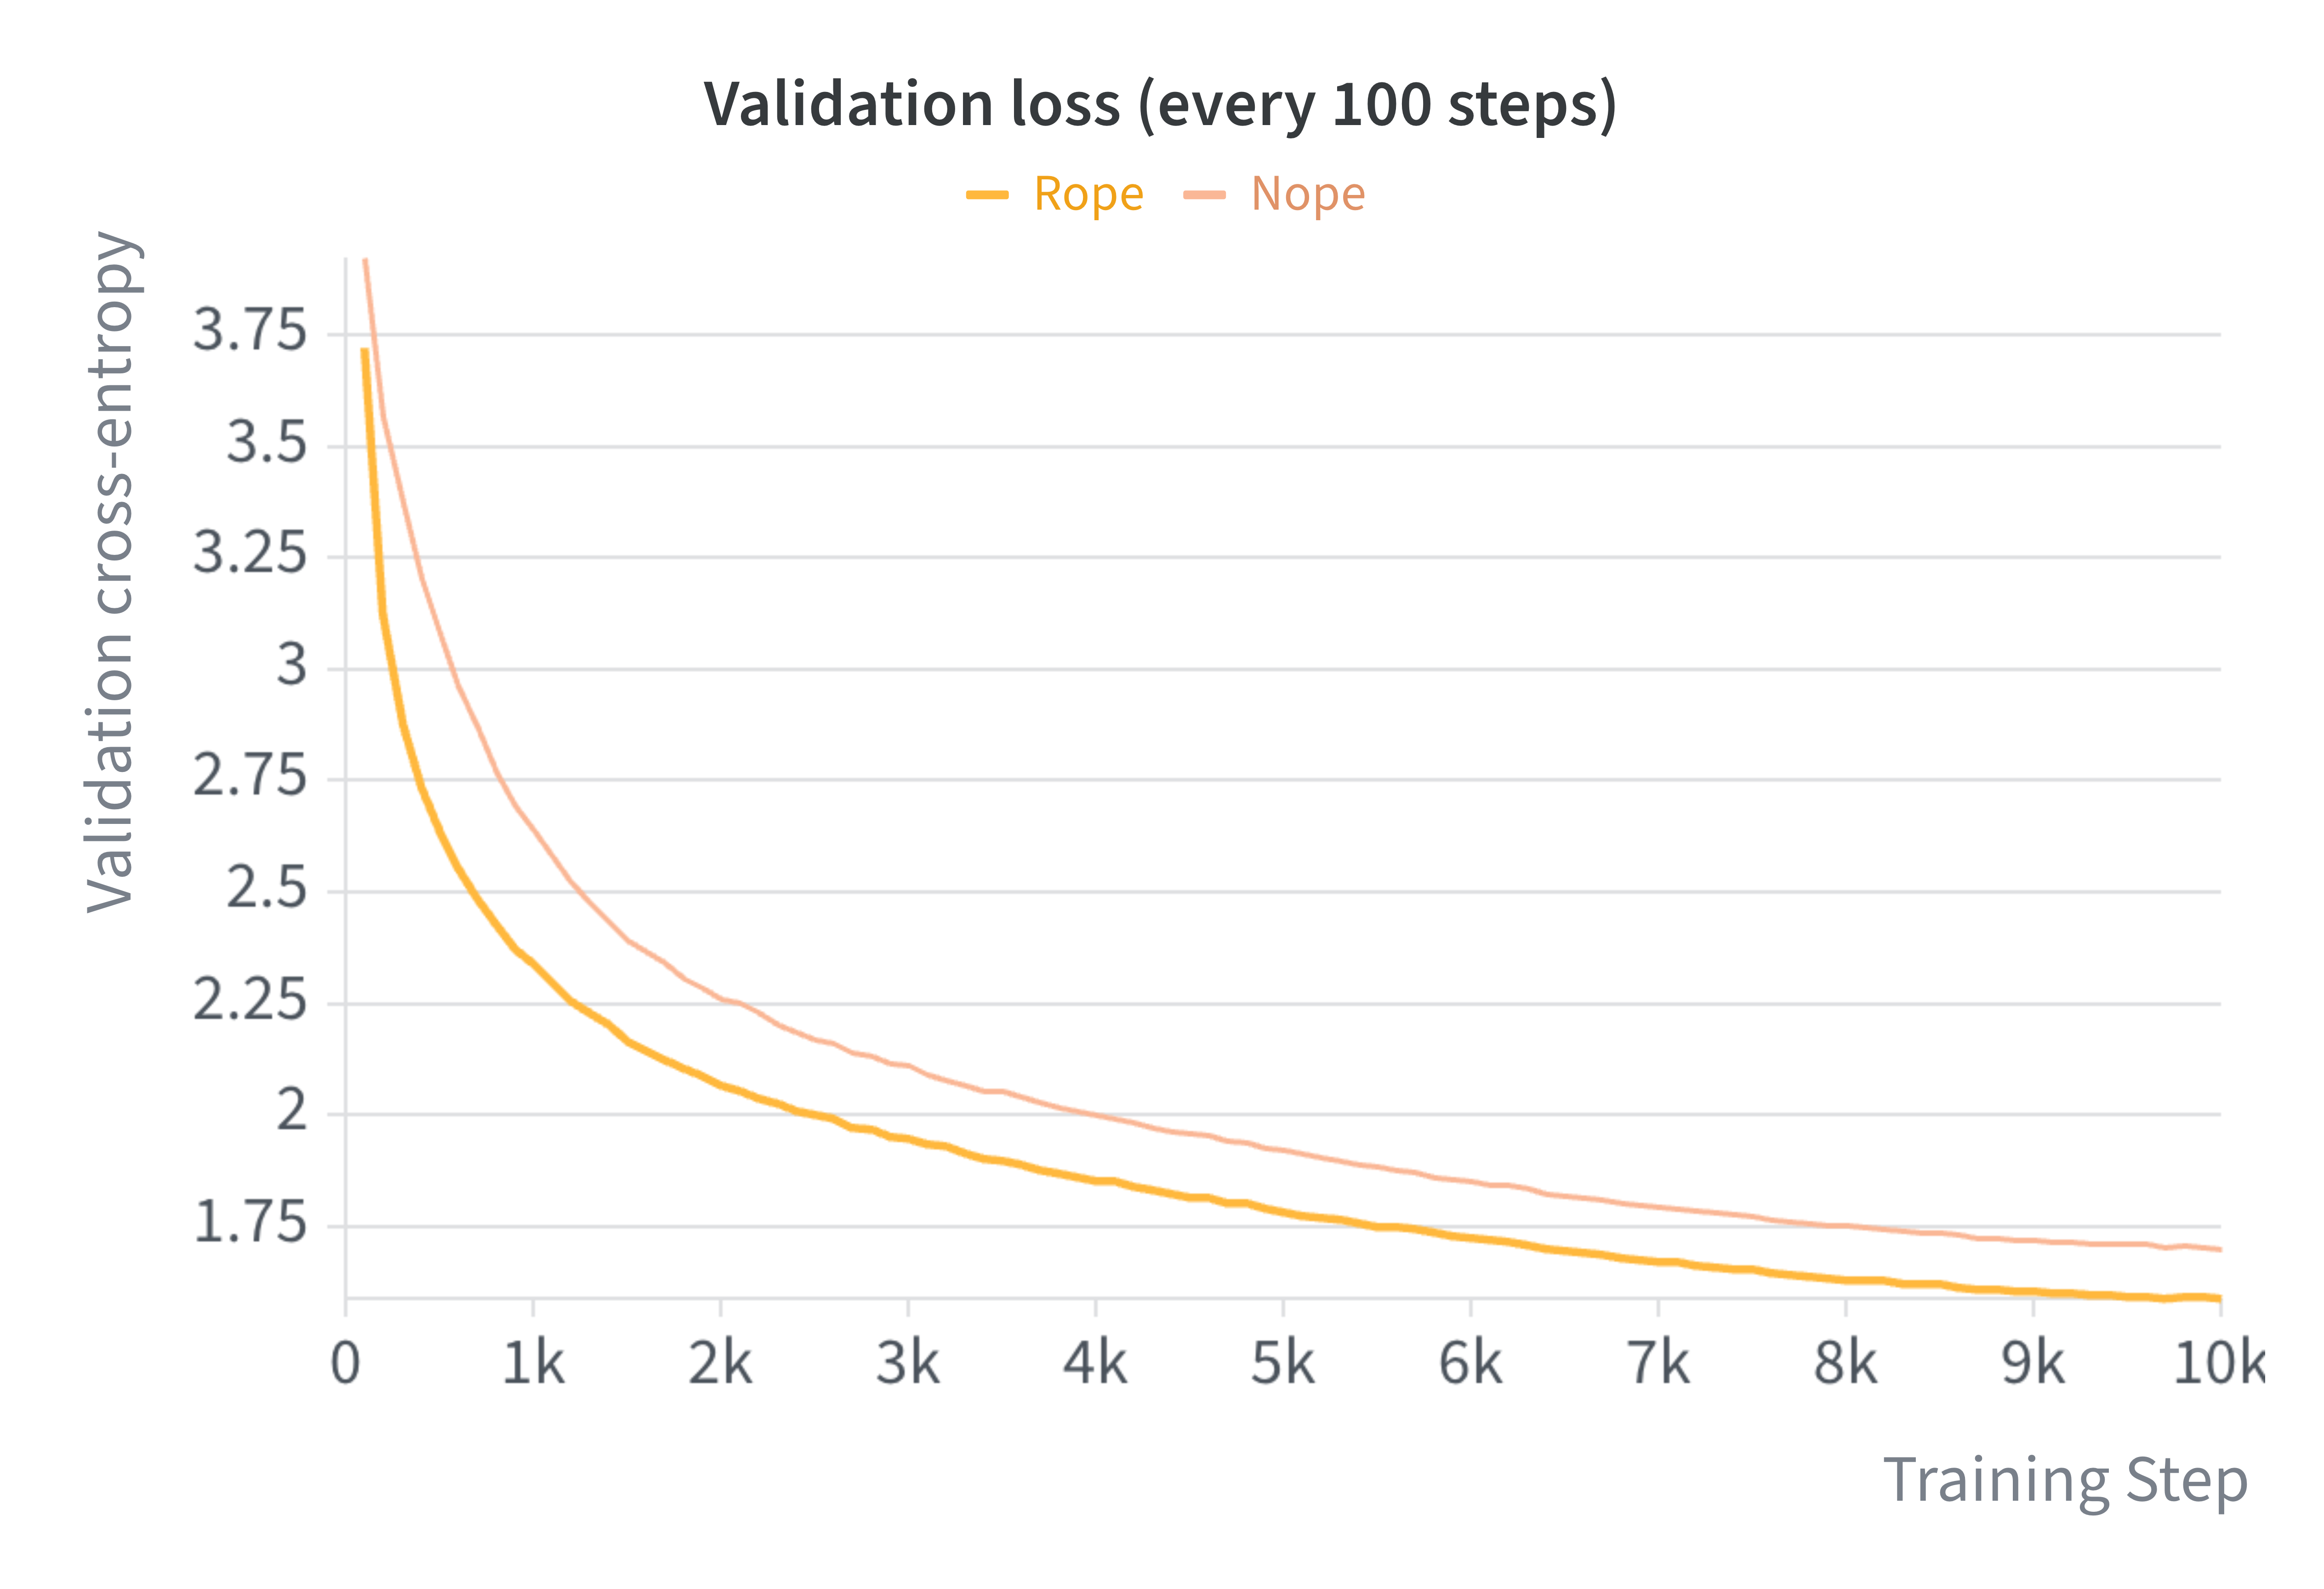
\includegraphics[width=0.49\textwidth]{figures/rope_nope_val.png}
    \caption{RoPE versus NoPE W\&B training loss (left) and validation loss
    (right). Both panels cover the full run; causal masking is present in
    both models.}
    \label{fig:nope_vs_rope}
\end{figure}

NoPE learned stably but had higher loss at all 100 matched evaluations.
It reached 1.7010 versus 1.5879 for RoPE, a gap of 0.1131, the largest
observed gap among these four architecture variants. Removing explicit
position information therefore hurt performance under this training budget.
The model still learned without RoPE; the result does not imply that a
causally masked Transformer cannot represent positional information.
These measurements concern context length 256 and do not test length
extrapolation or establish an optimal LR for NoPE.

\problem{swiglu\_ablation}{SwiGLU vs.\ SiLU}{1}

I replaced the gated feed-forward network with
$\operatorname{FFN}_{\mathrm{SiLU}}(x)=W_2\operatorname{SiLU}(W_1x)$.
The SiLU hidden width was $4d_{\mathrm{model}}=2048$, compared with 1344
for SwiGLU. This approximately matches the feed-forward parameter budget:
$2\times512\times2048=2{,}097{,}152$ versus
$3\times512\times1344=2{,}064{,}384$ weights per block.
Total model sizes were 22,827,520 and 22,696,448 parameters, respectively,
a difference of about 0.58\%. All other common settings were fixed.

\begin{figure}[H]
    \centering
    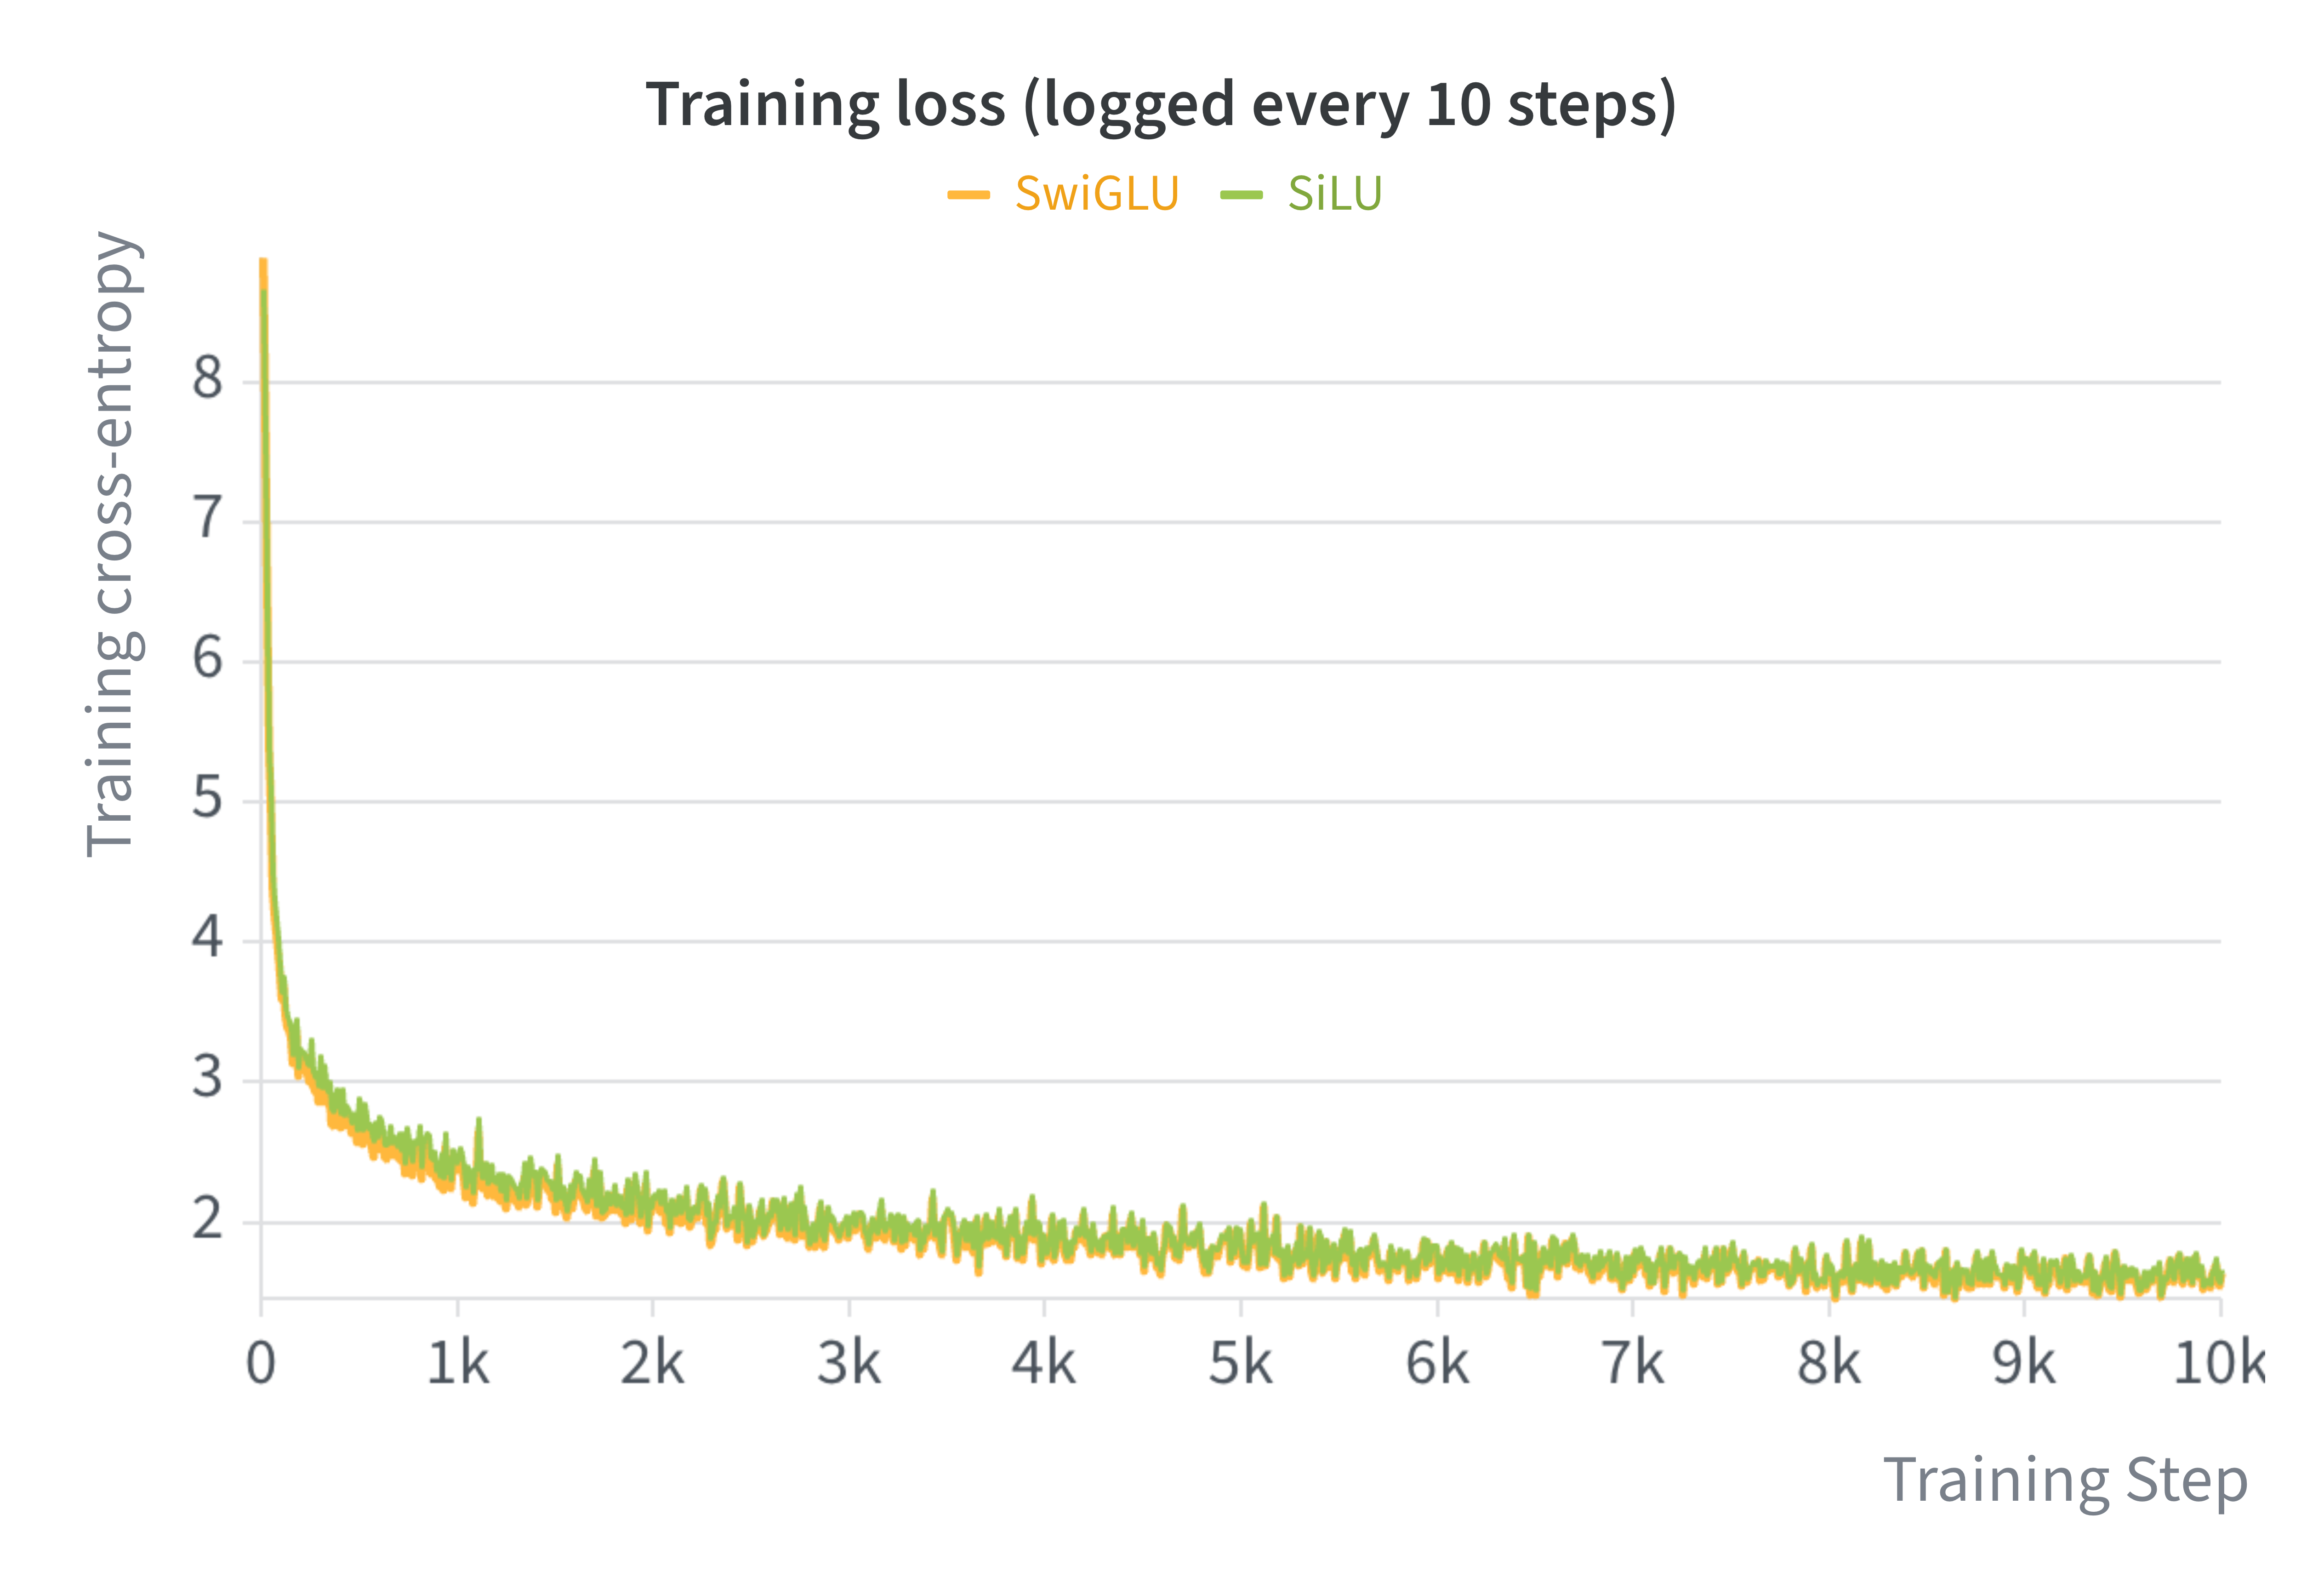
\includegraphics[width=0.49\textwidth]{figures/swiglu_silu_train.png}\hfill
    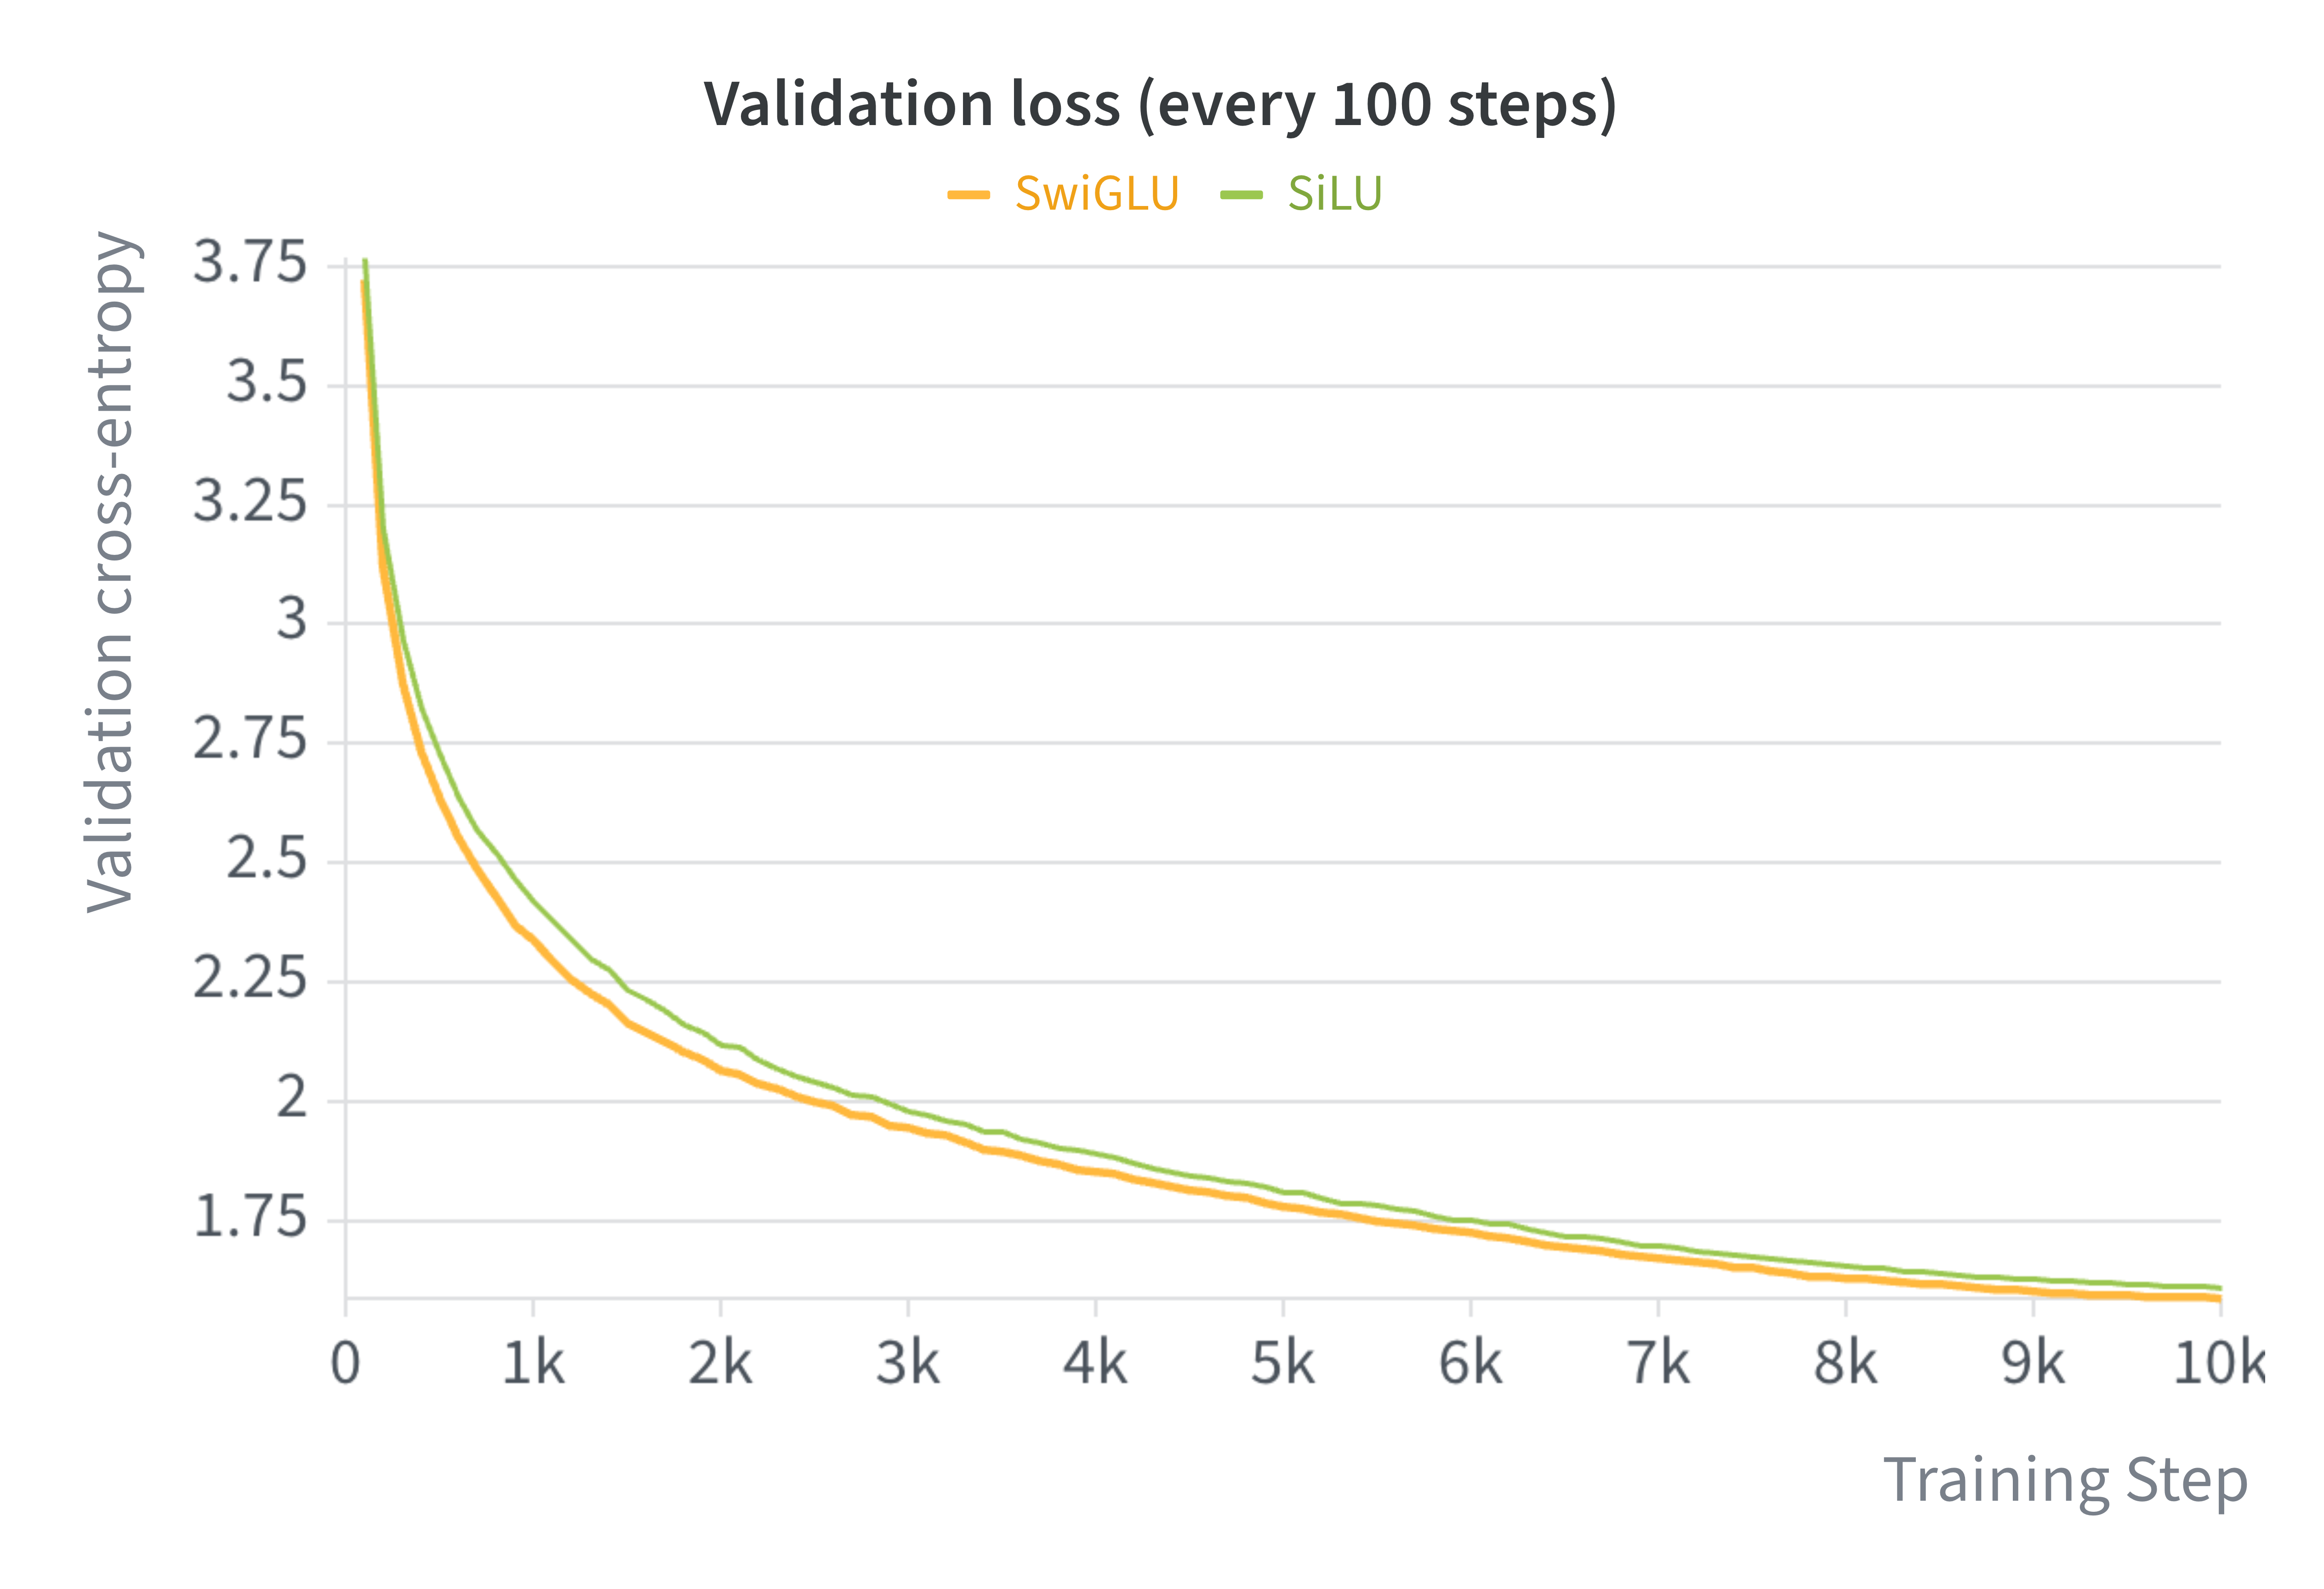
\includegraphics[width=0.49\textwidth]{figures/swiglu_silu_val.png}
    \caption{SwiGLU versus SiLU W\&B training loss (left) and validation loss
    (right), with approximately matched parameter counts. Orange denotes
    SwiGLU and green denotes SiLU in both panels.}
    \label{fig:swiglu_vs_silu}
\end{figure}

Both variants trained stably. SiLU had higher loss at every matched evaluation
and ended at 1.6106, compared with 1.5879 for SwiGLU, a gap of 0.0227.
The gated network performed modestly better in this run despite having
slightly fewer parameters, consistent with a benefit from gating at this
budget. Because only one seed and a shared LR schedule were tested, this
is an observed advantage for the chosen configuration, not a claim of
statistical significance or universal superiority.
